\documentclass[a4paper,12pt]{article}
\usepackage[utf8]{inputenc}
\usepackage[T1]{fontenc}
\usepackage[round]{natbib}
\bibliographystyle{humannat}
%\usepackage[sorting=nyt,citestyle=authoryear]{biblatex}
%\addbibresource{report.bib}
\usepackage[normalem]{ulem}
\usepackage[hidelinks]{hyperref}
\usepackage{libertine}
\usepackage[scaled=0.89]{inconsolata}
\usepackage[showframe=false,bottom=6em,head=8em]{geometry}
\usepackage[iso,danish]{isodate}
\usepackage{fancyvrb}
\usepackage{fancyhdr}
\usepackage{fancyref}
\usepackage{float}
\usepackage[dvipsnames]{xcolor}
\usepackage{tikz}
\usetikzlibrary{arrows.meta}
\usepackage{pgfplots}
\usepackage{pgfplotstable}
\pgfplotsset{compat=1.15}
\usepackage{amsmath}
\usepackage{amsfonts}
\usepackage{xfrac}
\usepackage{mathtools}

\pgfplotsset{compat=newest} % Allows to place the legend below plot
\usepgfplotslibrary{units} % Allows to enter the units nicely

\pagestyle{fancy}
\fancyhf{}
\lhead{FF501 Consensus in Distributed Systems}
\rhead{\today}
\chead{}
\lfoot{J. R. Fagerberg, M. Møller, L. O. J. Olsen, P. H. Ratgen, T. Stenhaug}
\cfoot{}
\rfoot{\thepage}
\renewcommand{\footrulewidth}{0pt}
\setcounter{secnumdepth}{2}
\setcounter{tocdepth}{2}

\date{\today}
\title{FF501 Consensus in Distributed Systems \vskip 0.3em
    \small{FF501, IMADA, University of Southern Denmark}
}
\author{
  Johan Ringmann Fagerberg - jofag17@student.sdu.dk\\
  Marcus Møller - moell17@student.sdu.dk \\
  Lucas Olai Jarlkov Olsen - luols17@student.sdu.dk\\
  Peter Heilbo Ratgen - perat17@student.sdu.dk\\
  Thomas Stenhaug - luols17@student.sdu.dk\\
  \\
  Advisor: Larisa Safina
}

\pagenumbering{roman}

\begin{document}

\maketitle

\setlength{\baselineskip}{1.44\baselineskip}

\begin{abstract}
Clock synchronization is a widely known problem that has many applications. E.g. multiple clients in a distributed system must agree on a single time in order to successfully tackle a problem. The problem has been worked on since the birth of computer networks, and solutions have evolved over time in response to changing demands. In recent years, consensus based algorithms have gained traction with the propagation of Internet of Things, and several new algorithms have been developed as a result.

We will compare two recent consensus-based algorithms for clock synchronization in distributed systems, Average TimeSynch (ATS) and Maximum Minimum Time Sync (MMTS), and implement them. The comparison will be based on the theoretical work from the algorithms' authors, our own analysis, and an implementation of both algorithms in virtual distributed networks.
\end{abstract}

\clearpage
\tableofcontents
\clearpage

\pagenumbering{arabic}
\setcounter{page}{1}

\section{Preface}

\section{Introduction}

The problem of time synchronization is one that is crucial to our modern day use of computers; many modern applications require a shared sense of time across multiple computers, whether that be for the sake of measuring the time it takes for messages to propagate throughout a network as in the case of e.g. computer games, or for the sake of ensuring that the order of events is consistent regardless of where in the network they occur, as in the case of e.g. banking or database transactions.

Even mechanical time synchronization is (or has been) a crucial part of our daily lives - the importance of having wall clocks agree on the current time across buildings, cities or even countries is a trivial example of time synchronization that predates even computers.

Time synchronization algorithms are many and varied, and have evolved over several decades. A recent development has been the introduction of consensus-based algorithms for distributed systems, in which a network of computing elements reach consensus on the current time without making use of central computing elements that hold more decision weight than others. In this paper we will be examining two such algorithms, Average TimeSynch (ATS) and Maximum Minimum Time Sync (MMTS).

\subsection{Distributed systems}

\begin{quote}
  A distributed system is a collection of autonomous computing
  elements that appears to its users as a single, coherent
  system.\cite{TanenbaumSteen06}
\end{quote}

Distributed systems are in essence networks of interconnected computing elements, capable of sending messages to each other. Characteristically, these computing elements are completely autonomous: although they may act on information provided by other computing elements, they are separate entities and have no knowledge of each others state beyond what is communicated to them.

The computing elements in a distributed system are usually called nodes, and each node is capable of communicating with a smaller subset of the system, the nodes that are known as its neighbors. To an outsider, a \textit{user} of the system, the distributed system appears as a single, unified entity \cite{TanenbaumSteen06}.

An example of a distributed system is a multi-player online game, where
the game environment is experienced as a single system, while there
are several nodes concerting the unified experience.  Another example
is the World Wide Web, which you can view as a large key-value store,
where Uniform Resource Locatiors (URL) are the key, and (typically)
HTML-pages are their value.  In the case of the WWW, both humans and
processes can considered users; indexing crawlers like Google are
examples of computer process users.

The type of distributed systems that ATS and MMTS are developed for are Wireless Sensor
Networks (WSNs).  Here the nodes are small, cheap devices, capable of communicating with each other wirelessly. Due to their low cost and small size, resulting in a low barrier of entry and a wide area of application, these devices have grown increasingly popular in recent years. However, due to the fragility of wireless communication and inexpensive hardware, these devices are prone to failure, resulting in a frequently changing distributed system structure\cite{SchenatoFiorentin11}.

\subsection{Consensus}
In a distributed system consisting of autonomous nodes, nodes must share some state. As the current time can be described as such a state, agreeing on, and propagating the agreed on state is the primary focus of time synchronization algorithms. The approaches are many and varied, but can usually be grouped into \textit{non-consensus-based algorithms} and \textit{consensus-based algorithms}.

In a consensus-based algorithm, each autonomous node is given equal weighting in the decision making process - the nodes are considered peers. In contrast, non-consensus-based algorithms frequently make use of a master-slave relationship between nodes, with the master deciding on the state without any input from slave nodes, and then pushing said state to its slaves - who in turn may have their own slaves, thus propagating the state throughout the network.

As this gives more decision making power to certain nodes, a consensus-based algorithm must take a different approach.

\subsection{Time synchronization} % Mostly done, might need to be split up

%Describe the time synchronization problem. Why is it necessary? Why is it not trivial?

Time synchronization is the problem of having a network of nodes agree on the value of their local clock at a given instant. It is an important part of any distributed system that requires some level of sequentiality of events. There are many different variants of the time synchronization problem, each with their own goals and disadvantages.

The most intuitive is the propagation of a "true" time throughout a network, as happens with our electronic devices today. For this approach one or more high-precision clock are seen as authoritative, and the value reported by them is propagated throughout the network and accepted at each node as the absolute truth. Unfortunately this is fragile to failed or malicious nodes near the root level. It is nonetheless the problem that must be solved if a known time must be propagated throughout the network.

An alternative problem is reaching consensus on a shared time in a network, regardless of what said time is. This is useful for ensuring sequentiality of events within the network, and can be made highly resistant to failed or malicious nodes in the network, as no nodes have a greater weight than others when it comes to reaching consensus on a value. As such this problem is highly applicable to scenarios where the reliability of the consensus is important, and where the impact of nodes joining or leaving the network must be limited. It is primarily this problem we will be discussing in this paper.

\subsubsection{Clock modelling}
%Clock drift

The hardware clock available to each node is often a low precision clock, whose time progression rate is not necessarily equal to that of other clocks. This means that over time, the output of the hardware clock will slowly drift away from other clocks. As the clock may have drifted considerably before the clock is observed, this also results in an initial time offset.

For the sake of modelling such a clock the concept of a virtual absolute time $t$ is introduced. This time is not known to any nodes, but is a useful tool, as it allows us to express the output of a given clock as a function of the current absolute time.

As such the local hardware clock $\tau$ of a node $i$ can be modelled as a linear function with two parameters, the skew $\alpha$ and the offset $\beta$:


\begin{equation}\label{eq:hardware-clock}
    \tau_i(t) = \alpha_i t + \beta_i.
\end{equation}

It is important to note that as $t$ is not known, neither $\alpha$ nor $\beta$ can be calculated directly. The only aspect of the hardware clock visible to the node is the output $\tau(t)$.

As the goal of clock synchronization is to find a way for every node in a network to report the same time at a given $t$ despite differing hardware clocks, equation \ref{eq:hardware-clock} must be transformed into a function that can be modified by the node. For this reason, the concept of logical clocks $L$ is introduced, defined as

\begin{align}
    L_i(t) &= \hat\alpha_i \tau_i(t) + \hat\beta_i \nonumber \\
        &= \hat\alpha_i \alpha_i t + \hat\alpha_i \beta_i + \hat\beta_i. \label{eq:logical-clock-expanded}
\end{align}

Modifying $\hat\alpha_i$ and $\hat\beta_i$ allows the node to change the output of the logical clock in relation to $t$, without knowing the parameters of the hardware clock $\tau$.

The goal of reaching consensus can thus be formalized in terms of logical clocks: As equation \ref{eq:logical-clock-expanded} makes clear, having two logical clocks $L_i$ and $L_j$ agree on the output at a given $t$ means having the parameters $\hat\alpha_i \alpha_i \approx \hat\alpha_j \alpha_j$ and $\hat\alpha_i \beta_i + \hat\beta_i \approx \hat\alpha_j \beta_j + \hat\beta_j$. Note that this does not mean that $\hat\alpha_i \approx \hat\alpha_j$, nor that $\hat\beta_i \approx \hat\beta_j$, as the parameters of the hardware clocks are likely to differ.

Expanding this to the entire network, reaching consensus can be formalized as reaching the point where $\hat\alpha_i \alpha_i \approx A$ and $\hat\alpha_i \beta_i + \hat\beta_i \approx B$, with $A$ and $B$ being network-global constants, for every node $i$ in the network.

%Time sync in 

\section{Strategies for time synchronization}

%Describe the advantages and disadvantages of the different kinds of time synchronization strategies (non-consensus vs. consensus)

By and large there are two ways of approaching the time synchronization problem, these being consensus and non-consensus based algorithms.

    \subsection{Non-consensus}
    %In general about non-consensus
    The non-consensus synchronization strategy is what we previously described as utilizing a very precise clock as a authoritative reference. The other clocks of the network change their clocks to match this "leader" clock.
    Examples of non-consensus time synchronization algorithms are The Berkeley algorithm, Reference Broadcast Synchronization (RBS), Timing-sync Protocol for Sensor Netorks (TPSN) and The Flooding Time Sync Protocol (FTSP). All of these algorithms incorporate some form of master-slave relationship. Regarding RBS, TPSN and FTSP, these are tailored to Wireless Sensor Networks (WSN).
    
    %Not sure if it should be included
    \paragraph{The Berkeley algorithm} The simplest algorithms is the Berkeley algorithm, as describes by \citet{Gusella89}, the algorithm works by having a centralized time server polling the nodes for their current clock value. The time server then averages these clock values, along with its own clock value. The time server then instructs each node to adjust to the averaged clock value. 

    \paragraph{RBS} The Reference Broadcast Synchronization algorithm, described by \citet{ElsonGirodEstrin02},  functions by a central node sending out a reference packet to each node. Each node then records the time at which the reference packet was received. %Exhanging of recorded clock times? 
    The nodes should then compare their results. This is done by calculating their offset relative to another receiver. The offset is calculated by 
    \begin{equation}
        \label{offsetcalc}
        \textit{Offset} [i,j] = \frac{1}{M}\sum^M_{k=1} (T_{j,k} - T_{i,k})
    \end{equation}
    where $i$ and $j$ are two nodes and $T_{j,k}$ is $j$'s clock when it received broadcast $k$. $M$ is the number of reference broadcasts.  %Handling of clock skew. Using post-factosynchronization
    However calculating the offset of a node's clock relative to another, and vice versa is not enough, as it doesn't take clock drift into account. The offset can then be calculated a function by utilzing linear regression. 
    $$\textit{Offset}[i,j](t) = \alpha t + \beta$$
    The node then stores this information about the node's relative drift between its clock and any other node in the network (of which is it maintains a relative clock). This creates clusters of synchronized nodes, which all are connected to the root node.
    
    \paragraph{TPSN} The Timing-sync Protocol for Sensor Networks protocol, described by \citet{GaneriwalEtAl03}, functions by selecting a node as the root node. At first the algorithm enters the "level discovery phase", in this  phase each node is assigned a level. This is done the root node sending out a \texttt{level\_discovery} packet. Then each node assigns itself to a level lower than from which at received the packet. This node then broadcasts a \texttt{level\_discovery} packet. The algorithm then enters the synchronization phase, it uses sender-receiver synchronization. This sets it apart from RBS, which uses receiver-receiver synchronization. This mean that the receiver synchronizes to the sender. The time is synchronized by calculating the clock drift and the propagation time between nodes. As seen on figure \ref{timemeasuretpsn}, the receiver node A sends a synchronization pulse to the sender B, which is located at a greater level. Node A sends a synchronization pulse to B, which in turn sends back an acknowledgement packet. This acknowledgement packet contains the values of $T_1$, $T_2$ and $T_3$. Then the final time $T_4$ is recorded by node A. From these values the clock drift ($\Delta$) and propagation delay ($d$) between the two nodes can be calculated. 
    
    $$\Delta = \frac{(T_2-T_1) - (T_4 - T_3)}{2} \quad ; \quad d = \frac{(T_2-T_1) + (T_4-T_3)}{2}$$
    
    \begin{figure}[H]
        \centering
        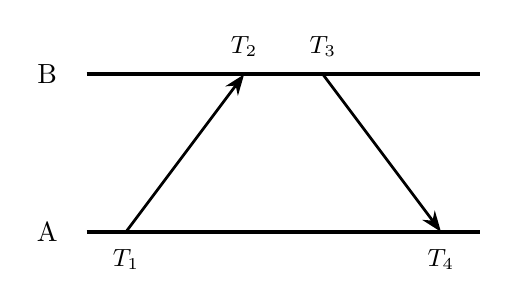
\begin{tikzpicture}
            \draw [line width = 1.5pt](0,0) node (upper-line-start){}
                  -- (5,0) node (upper-line-end){};
            \draw [line width = 1.5pt](0,-2) node (lower-line-start){}
                  -- (5,-2) node (lower-line-end){};
            \node [left of = upper-line-start, node distance = 0.5cm](){B};
            \node [left of = lower-line-start, node distance = 0.5cm](){A};
            \draw [arrows={-Stealth[length = 7.5pt]}, line width = 1pt] (0.5,-2) node (first-line-start){}
                  -- (2,0) node (first-line-end){};
            \draw [arrows={-Stealth[length = 7.5pt]}, line width = 1pt] (3,0) node (last-line-start){}
                  -- (4.5,-2) node (last-line-end){};
            \node [below of = first-line-start, node distance = 0.35cm] (){\small $T_1$};
            \node [above of = first-line-end, node distance = 0.35cm] (){\small $T_2$};
            \node [above of = last-line-start, node distance = 0.35cm] (){\small $T_3$};
            \node [below of = last-line-end, node distance = 0.35cm] (){\small $T_4$};
         \end{tikzpicture}
         \caption{A model of communication between nodes. $T_1$ and $T_4$ are recorded on the clock of node A, and $T_2$ and $T_3$ on the clock of node B}
        \label{timemeasuretpsn}
    \end{figure}
    
    In general the synchronization is initiated by the root node. By instructing level 1 nodes to synchronize to the root node. When the level 1 nodes are synchronized, the level 2 nodes are synchronized and so forth. 
    
    
    \paragraph{FTSP} %allegedly one of the best non-consensus algorithms
    The Flooding Time Sync Protocol, is described by \citet{Maroti04}. The objective of the Flooding Time Sync Protocol is to achieve synchronization of the clocks of the participating nodes. As opposed to TPSN, FTSP keeps an ad-hoc structure of the nodes. 
    
    \begin{figure}[H]
        \centering
        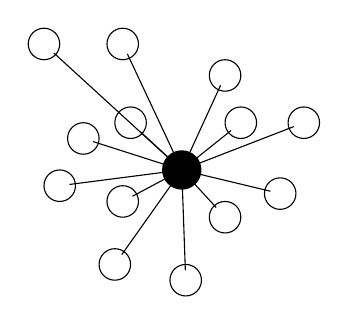
\begin{tikzpicture}
        
        \filldraw[fill=white, draw=black] (0,-1) circle (0.2cm) node(1){};
        \filldraw[fill=white, draw=black] (3.0,-2.9) circle (0.2cm) node(2){};
        \filldraw[fill=white, draw=black] (3.3,-2) circle (0.2cm) node(3){};
        \filldraw[fill=white, draw=black] (2.5,-2) circle (0.2cm) node(4){};
        \filldraw[fill=white, draw=black] (2.3,-1.4) circle (0.2cm) node(5){};
        \filldraw[fill=white, draw=black] (1,-1) circle (0.2cm) node(6){};
        \filldraw[fill=white, draw=black] (0.5,-2.2) circle (0.2cm) node(7){};
        \filldraw[fill=white, draw=black] (1,-3) circle (0.2cm) node(8){};
        \filldraw[fill=white, draw=black] (1.8,-4) circle (0.2cm) node(9){};
        \filldraw[fill=white, draw=black] (2.3,-3.2) circle (0.2cm) node(10){};
        \filldraw[fill=white, draw=black] (1.1,-2) circle (0.2cm) node(11){};
        \filldraw[fill=white, draw=black] (0.2,-2.8) circle (0.2cm) node(12){};
        \filldraw[fill=white, draw=black] (0.9,-3.8) circle (0.2cm) node(13){};
        \fill [black](1.75,-2.6) circle (0.25cm) node(main){};
        
        \draw (1) -- (main);
        \draw (2) -- (main);
        \draw (3) -- (main);
        \draw (4) -- (main);
        \draw (5) -- (main);
        \draw (6) -- (main);
        \draw (7) -- (main);
        \draw (8) -- (main);
        \draw (9) -- (main);
        \draw (10) -- (main);
        \draw (11) -- (main);
        \draw (12) -- (main);
        \draw (13) -- (main);
        
        \end{tikzpicture}
        \caption{Illustration of an ad-hoc network structure, with 14 nodes of which one is the leader.}
    \end{figure}
    %Time-stamping
    The FTSP uses a radio broadcast, which contains the transmitter's time stamp. Upon receiving the broadcast the local time is recorded. The receiver then calculates its bit offset, so it can interpret the data from the transmitter correctly. The data is then followed by some check bytes called CRC bytes. FTSP has a different way of time stamping than TPSN (which time stamps at MAC layer). The FTSP time stamps seeks to reduce irregularities in the handling of interrupts and encoding and decoding. Irregularities occur in the handling of interrupts, when interrupts are disabled for a short period of time on the receiving microcontroller. The irregularities is reduced by taking the minimum of the time stamps. This approach results in a time stamping accuracy of $1.4 \mu \text{s}$ between transmitters and receivers.
    
    %Management of clock drift
    
    As we know the oscillation of a quartz crystal can be irregular. And clocks will drift apart relative to each other after some time. To maintain the previously mentioned accuracy of a few microseconds, continuous and frequent synchronization would be required. Instead of having a high synchronization frequency, which would congest the network. The approach of estimating the offset of the local clock relative to the global time, was chosen. This is done by applying linear regression to the offset, between the clock of the local node and the clock of the transmitter, relative to time passed. Thus the offset can be estimated. In an experiment conducted in the paper, with a time synchronization interval of 30 seconds and a query interval of 18 seconds, the average error was $1.48 \mu \text{s}$.
    
    %Multihop synchronization
    
    \subsection{Consensus}
    %Description of Consensus as a concept here.
    Consensus based synchronization strategies do not utilize a reference node to correctly synchronize nodes \cite{HeLiChenCheng13}. Instead these protocols are completely distributed and can be utilized in more dynamic network topologies without a common root.
    
    To analyze the consensus-based algorithms, Average Time Synchronization (ATS) and Modified Maximum Time Synchronization (MMTS), we researched their creation and how they function. The following sections describe these algorithms to provide a basis of knowledge before their comparison.
    
    \paragraph{ATS} The Average Time Synchronization, as described by \citet{SchenatoFiorentin11}, uses three important operations to achieve it's synchronization between nodes in the network: Relative drift estimation, drift compensation and offset compensation. The algorithm utilizes a pseudo-periodic broadcast as it's communication protocol between nodes. The nodes each transmits a set of information to all of it's neighbors with a period $\mathrm{T}$. The instants in which the nodes transmit is defined as 
    
    \begin{equation}
        t^i_\ell = \frac{\ell\mathrm{T} - \beta_i}{\alpha_i} = \ell\mathrm{T}_i + \bar{\beta_i},
    \end{equation}
    or $\tau_j(t^i_\ell) = \ell\mathrm{T}$, where i is the node and $\ell \in N$ is the message number. Each node transmits it's message at every period $\mathrm{T}$ based on its own clock which it doesn't share with it's neighbors. Meaning the transmission instants are different for each node due to the different $\alpha_i$ in the nodes. The broadcast is therefore pseudo-periodic.
    
    
    The relative drift estimation estimates the difference in clock rate, or relative drift, between each node's clock i compared to their neighbor j. Clock drift  Every node i estimates the drift between it and all of it's neighbors. Part of the aforementioned set of information sent in messages between nodes, is the current local time of the sender, node j, denoted by $\tau_j(t^j_\ell)$. When node i receives the message it records it's own local time by $\tau_i(t^j_\ell)$. Node i stores the two clock readings as $(\tau^{old}_{i_j}, \tau^{old}_j) = (\tau_i(t^j_\ell), \tau_j(t^j_\ell))$. 
    When i later receives another message from j, the process repeats and a new clock reading pair is constructed, $(\tau_i(t^j_{\ell + 1}), \tau_j(t^j_{\ell + 1}))$. Finally the estimate of $\alpha_{ij} = \frac{\alpha_j}{\alpha_i}$ is found by a low-pass filter as described below.
    
    \begin{equation}
        \begin{rcases*}
            (\tau_{ij}^{new}, \tau_j^{new}) &= $(\tau_i(t^j_\ell), \tau_j(t^j_\ell))$ \\
            \eta_{ij}(t^+) &= $\rho_\eta\eta_{ij}(t) + (1 - \rho_\eta)\frac{\tau_j^{new} - \tau_j^{old}}{\tau_{ij}^{new} - \tau_{ij}^{old}} $ \\
            (\tau_{ij}^{old}, \tau_j^{old}) &= $(\tau_{ij}^{new}, \tau_j^{new})$
        \end{rcases*} \nonumber
    \end{equation}
    \begin{equation}
        t = t^j_\ell
    \end{equation}
    
    \begin{equation}
        \eta_{ij}(t) = \eta_{ij}(t^+),\ t \in (t^+, t_{\ell + 1}^j]
    \end{equation}
    
    Where $\rho_\eta \in (0, 1)$ is a tuning parameter, and $t^+$ is the clock update. $\eta_{ij}$ converges towards $\alpha_{ij}$ thereby making (5) and (6) a valid way to estimate the skew difference between two nodes and allowing us to align them.
    
    Drift compensation is what follows the estimation. Each node stores its own estimate of the global clock rate and uses this estimate in the compensation to reach a common clock rate $\bar{\alpha}$. The algorithm then messages it's neighbors and uses the received information, to average it's estimate with the estimate of its neighbors. When a message is sent from node i to node j at time $t^j_\ell$ it changes it's own estimate value $\hat{\alpha}$ by doing
    
    \begin{equation}
        \hat{\alpha_i}(t^+) = \rho_v\hat\alpha_i(t) + (1 - \rho_v)\eta_{ij}(t)\hat\alpha_j(t), \ t = t^j_\ell, \ i \in \mathcal{N}_j.
    \end{equation}
    
    $\alpha_j$ is the global clock drift estimation of node j. When each node periodically averages its drift estimate with it's neighbors, it follows that all estimates $\hat\tau_i(t)$ will ultimately have the same speed.
    
    
    Offset Compensation is the final major operation of ATS. After each node has reached consensus on their drift estimation all that is left to reach complete synchronization, is to fix the offset between the clocks. An algorithm to fix any such remaining offsets is applied. The subsequent equation describes this adjustment.
    
    \begin{equation}
        \hat{o}_i(t^+) = \hat{o}_i(t) + (1 - \rho_o)(\hat{\tau}_j(t) - \hat{\tau}_i(t)), \ t=t^j_\ell,i \in \mathcal{N}_j.
    \end{equation}
    
    Each node computes the estimated clock difference $\hat\tau_j(t) - \hat\tau_i(t)$ and attempts to adjust it's own clock offset to minimize this difference. The offset compensation is not required to wait for the drift compensation to finish synchronizing all the clock speeds. Instead it is applied simultaneously, yielding a better performance and quicker convergence.  
    
    \paragraph{MMTS} The Maximum Minimum Time Synchronization algorithm aims to make all clocks in the distributed system converge to a unified clock. The time of said unified clock may not be the actual time, but reaching a consensus is often more crucial than staying close to the actual time.
    The method to converge that MMTS uses is that each node in the network will, at a certain interval, broadcast it's time to the neighbours. Upon receival of such a message, the node will compute a skew that is relative to the previous message received from that sender:
    \begin{equation}
        \alpha_{ij}(k) = \frac{\frac{\tau_j(t_k) - \tau_j(t_{k-1})}{\tau_i(t_k)-\tau_i(t_{k-1})} + (k-1)\alpha_{ij}(k-1)}{k}
    \end{equation}

    Where \textit{i} is the computing node, \textit{j} is the node that sent the message, \textit{$\tau$} is the hardware time at the time of a message, and \textit{k} is the amount of messages received from that node.
    
    Then, the maximum skew and the maximum offset as well as the minimum counterparts are computed.
    
    \begin{equation}
        \hat{\alpha}_{imax} = \hat{\alpha}_i + \mu_i
    \end{equation}
    
    \begin{equation}
        \hat{\beta}_{imax} = \hat{\beta}_i + \nu_i
    \end{equation}
    
    \begin{equation}
        \hat{\alpha}_{imin} = \hat{\alpha}_i - \mu_i
    \end{equation}
    
    \begin{equation}
        \hat{\beta}_{imin} = \hat{\beta}_i - \nu_i
    \end{equation}
    
    Using these, $p_{ij}(k)$ and $q_{ij}(k)$ are computed, which in turn determines whether to use maximum or minimum consensus for the computation of the given message.
    
    \begin{equation}
        p_{ij}(k) = \frac{a_{ij}(k)(\hat{\alpha}_j + \mu_j)}{\hat{\alpha}_{imax}}
    \end{equation}
    
    \begin{equation}
        q_{ij}(k) = \frac{\alpha_{ij}(k) (k) (\hat{\alpha}_j - \mu_j)}{\hat{\alpha}_{imax}}
    \end{equation}
    
    Now, there are two consensus evaluations being done, based on $p_{ij}(k)$ and $q_{ij}(k)$. The first is maximum consensus and goes as follows:
    
    If $p_{ij}(k)$ is greater than 1, then:
    
    \begin{equation}
        \hat{\alpha}_{imax} = \alpha_{ij}(k)(\hat{\alpha}_j + \mu_j)
    \end{equation}
    
    \begin{equation}
        \hat{\beta}_{imax} = (\hat{\alpha}_j + \mu_j) \tau_j(t_k) + \hat{\beta}_j + \nu_j - \alpha_{ij}(k)(\hat{\alpha}_j + \mu_j) \tau_i(t_k)
    \end{equation}
    
    Or, if $p_{ij}(k)$ is exactly 1:
    
    \begin{equation}
        \hat{\beta}_{imax} = \max{_l} = \prescript{}{ij}{\{ ( \hat{\alpha}_l + \mu_l ) \tau_l(t_k) \}} - ( \hat{\alpha}_i + \mu_i ) \tau_i(t_k)
    \end{equation}
    
    On the other hand, there is the minimum consensus, which evaluates $q_{ij}(k)$. If $q_{ij}(k)$ is greater than 1, then:
    
    \begin{equation}
        \hat{\alpha}_{imin} = \alpha_{ij}(k)(\hat{\alpha}_j - \mu_j)
    \end{equation}
    
    \begin{equation}
        \hat{\beta}_{imin} = ( \hat{\alpha}_j - \mu_j ) \tau_j(t_k) + \hat{\beta}_j - \nu_j - \alpha_{ij}(k)(\hat{\alpha}_j - \mu_j)\tau_i(t_k)
    \end{equation}
    
    Or, in the case of $q_{ij}(k)$ being equal to 1:
    
    \begin{equation}
         \hat{\beta}_{imin} = \min{_l} = \prescript{}{ij}{\{ ( \hat{\alpha}_l - \mu_l ) \tau_l(t_k) + \hat{\beta}_l - \nu_l \}} - ( \hat{\alpha}_i - \mu_i ) \tau_i(t_k) 
    \end{equation}
    
    Finally, $[\tau_i(t_{k-1}), \tau_j(t_{k-1},\alpha_{ij})]$ is replaced by $[\tau_i(t_k), \tau_j(t_k),\alpha_{ij}(k)$ such that upon receival of the next message, a new relative skew will be computed with relation to this one.
    
    
%Describe algorithms Average TimeSync and Modified Maximum Time Sync.

\section{Analysis}
%Analyze the consensus-based algorithms Average TimeSync and Modified Maximum Time Sync. 
%Compare the algorithms, their advantages and disadvantages, and their areas of application (through both %implementation and theoretical analysis).

In this section we analyze different strategies of clock synchronization. We discuss consensus-based strategies versus non-consensus strategies, describing their advantages and disadvantages. We also analyze ATS and MMTS and analyze their advantages and disadvantages in different areas of application.

\subsection{Non-consensus vs. Consensus}

\paragraph{Changes in network topology} As stated earlier there are several key differences between non-consensus and consensus based algorithms. As stated by \cite{SchenatoGamba07}, consensus based time synchronization algorithms are more resistant to node failure, as they are fully distributed. This differs from non-consensus based algorithms, which are less robust, regarding node failure and node appearance. This is the case in all non-consensus, where a new node needs to be elected as the leader. As shown by \citet{HeLiChenCheng13} MTS (of which MMTS is a variant) a restarted node synchronizes after 2 synchronization cycles, thus the synchronization is not affected. The same pattern is followed when a new node joins the network.

\paragraph{Organization of nodes} The non-consensus algorithms also have different way of organizing nodes, eg. RBS has an ad hoc approach, where the receiving nodes are synchronized relative to one another. TPSN has a spanning tree based approach. And FTSP has an ad hoc approach. Having an ad hoc approach saves time building a spanning tree, and is more resistant to node and connection failures. This is not an issue a completely distributed consensus algorithm.

\paragraph{Scalability}

WSN can be of significant scale (150+ nodes). For an algorithm to be applicable in such a large network it needs to be shown to do so. TPSN has been shown to work in a large scale network of 150 to 300 nodes. As specified by \cite{GaneriwalEtAl03}, the performance is due to networks hierarchical structure, as it is possible to find a shortest path to each node. And by using multihop it's possible to communicate to each node, however this introduces synchronization errors and the larger the hop, the larger the error. 

\paragraph{Performance}
    
\cite{Sundararaman05} 


\subsection{Average Time Synchronization Protocol}
According to \citet{SchenatoFiorentin11}, one of the weaknesses of ATS is it's inaccuracy when utilizing it on larger networks. The further the "hop distance", that is the path from one node to another through it's neighbors, the greater the error of synchronization. However the error between adjacent nodes is said to only be weakly affected by the size of the network. ATS' performance is said to worsen for long synchronization periods. Compared to FTSP, ATS is shown to have a slightly better performance. It also exhibits a consistent lowering of synchronization error while FTSP often has sudden irregular spikes in error.


In \citet{HeChengShiChen13}, a paper suggesting a more secure version of ATS, ATS' is demonstrated to have significant weaknesses when errors are caused deliberately. It describes how planted attack nodes can thoroughly worsen it's performance and even prevent synchronization completely. An attack node would be able to freely alter it's own hardware clock and send false messages to it's neighbors, thereby hindering the synchronization process. An attack node essentially has complete control over it's neighbors. When it receives a message with it's neighbors skew it can use this reading and it's own ability to freely alter it's hardware clock to control what it's neighbors computes as it's estimated average.



\section{Results}

In an effort to empirically compare ATS and MMTS we implemented a virtual network capable of simulating a communication delay $\lambda$ between nodes. We implemented ATS and MMTS in this virtual network, and simulated ten seconds of algorithm execution while gathering data on algorithm performance.

For this purpose we introduce the concept of an average synchronization error $\overline{E}(t)$ of a set of nodes $\boldsymbol{N}$, defined as the average distance from each node's logical clock to the average of every logical clock $\overline{L}(t)$ $$\overline{E}(t) = \frac{1}{|\boldsymbol{N}|} \cdot \sum_{i \in \boldsymbol{N}} \left| L_i(t) - \overline{L}(t) \right|$$

This value is calculated every 100 milliseconds of algorithm execution. The resulting data set is averaged with five other data sets of the same algorithm with the same parameters to gain a fair representation of algorithm performance.

For the data presented below, the tuning parameters of ATS were set to $\rho_\eta = \rho_v = \rho_o = 1 / 2$. The nodes in the virtual network were arranged in a $5\times5$ grid, with each node being able to send messages to their immediate neighbors.

\subsubsection{Performance at varying communication delays}
By varying the communication delay $\lambda$ of our simulation, while keeping the broadcasting interval $T$ constant at $T = 100 \text{ms}$, we were able to compare algorithm performance at various levels of latency.

It is clear from figures \ref{fig:ats-latency} and \ref{fig:mmts-latency} that while ATS is heavily impacted by an increase in latency, MMTS is largely unaffected. As such, high latency leads to ATS performing relatively worse compared to MMTS, while they have comparable performance at $0$ latency.

\begin{figure}[p!h]
    \centering
    \begin{tikzpicture}
      \begin{axis}[
          %width=\linewidth, % Scale the plot to \linewidth
          grid=major, % Display a grid
          grid style={dashed,gray!30}, % Set the style
          xlabel=Time $t$, % Set the labels
          ylabel=Average error $\overline{E}(t)$,
          xmin=0,
          xmax=10000,
          ymin=0,
          x unit=ms, % Set the respective units
          y unit=ms
        ]
        \addplot+[mark=none, ultra thick] table[x=Time,y=Error,col sep=comma] {../data/ats-0-100.csv}; 
        \addplot+[mark=none, ultra thick] table[x=Time,y=Error,col sep=comma] {../data/ats-10-100.csv}; 
        \addplot+[mark=none, ultra thick] table[x=Time,y=Error,col sep=comma] {../data/ats-50-100.csv}; 
        
        \legend{$\lambda = 0 \text{ms}$,$\lambda = 10 \text{ms}$,$\lambda = 50 \text{ms}$}
      \end{axis}
    \end{tikzpicture}
    \caption{ATS performance at various communication delays $\lambda$} \label{fig:ats-latency}
    
    \vspace*{6em}
    
    \begin{tikzpicture}
      \begin{axis}[
          %width=\linewidth, % Scale the plot to \linewidth
          grid=major, % Display a grid
          grid style={dashed,gray!30}, % Set the style
          xlabel=Time $t$, % Set the labels
          ylabel=Average error $\overline{E}(t)$,
          xmin=0,
          xmax=10000,
          ymin=0,
          x unit=ms, % Set the respective units
          y unit=ms
        ]
        \addplot+[mark=none, ultra thick] table[x=Time,y=Error,col sep=comma] {../data/mmts-0-100.csv}; 
        \addplot+[mark=none, ultra thick] table[x=Time,y=Error,col sep=comma] {../data/mmts-10-100.csv}; 
        \addplot+[mark=none, ultra thick] table[x=Time,y=Error,col sep=comma] {../data/mmts-50-100.csv}; 
        
        \legend{$\lambda = 0 \text{ms}$,$\lambda = 10 \text{ms}$,$\lambda = 50 \text{ms}$}
      \end{axis}
    \end{tikzpicture}
    \caption{MMTS performance at various communication delays $\lambda$} \label{fig:mmts-latency}
\end{figure}

\begin{figure}[p!h]
    \centering
    \begin{tikzpicture}
      \begin{axis}[
          %width=\linewidth, % Scale the plot to \linewidth
          grid=major, % Display a grid
          grid style={dashed,gray!30}, % Set the style
          xlabel=Time $t$, % Set the labels
          ylabel=Average error $\overline{E}(t)$,
          xmin=0,
          xmax=10000,
          ymin=0,
          x unit=ms, % Set the respective units
          y unit=ms
        ]
        \addplot+[mark=none, ultra thick] table[x=Time,y=Error,col sep=comma] {../data/ats-10-20.csv}; 
        \addplot+[mark=none, ultra thick] table[x=Time,y=Error,col sep=comma] {../data/ats-10-100.csv}; 
        \addplot+[mark=none, ultra thick] table[x=Time,y=Error,col sep=comma] {../data/ats-10-500.csv}; 
        
        \legend{$T = 20 \text{ms}$,$T = 100 \text{ms}$,$T = 500 \text{ms}$}
      \end{axis}
    \end{tikzpicture}
    \caption{ATS performance at various broadcasting intervals $T$} \label{fig:ats-interval}
    
    \vspace*{6em}

    \begin{tikzpicture}
      \begin{axis}[
          %width=\linewidth, % Scale the plot to \linewidth
          grid=major, % Display a grid
          grid style={dashed,gray!30}, % Set the style
          xlabel=Time $t$, % Set the labels
          ylabel=Average error $\overline{E}(t)$,
          xmin=0,
          xmax=10000,
          ymin=0,
          x unit=ms, % Set the respective units
          y unit=ms
        ]
        \addplot+[mark=none, ultra thick] table[x=Time,y=Error,col sep=comma] {../data/mmts-10-20.csv}; 
        \addplot+[mark=none, ultra thick] table[x=Time,y=Error,col sep=comma] {../data/mmts-10-100.csv}; 
        \addplot+[mark=none, ultra thick] table[x=Time,y=Error,col sep=comma] {../data/mmts-10-500.csv}; 
        
        \legend{$T = 20 \text{ms}$,$T = 100 \text{ms}$,$T = 500 \text{ms}$}
      \end{axis}
    \end{tikzpicture}
    \caption{MMTS performance at various broadcasting intervals $T$} \label{fig:mmts-interval}
\end{figure}

\subsubsection{Performance at varying broadcasting intervals}
By varying the broadcasting interval $T$ of the algorithms, while keeping the communication delay $\lambda$ constant at $\lambda = 10 \text{ms}$, we were able to compare algorithm performance at various levels of bandwidth.

Unlike the communication delay, both algorithms are significantly affected by changes in the broadcasting interval as shown by figures \ref{fig:ats-interval} and \ref{fig:mmts-interval}. Although MMTS still reaches stable synchronization quicker than ATS, the relative performance of the algorithms is significantly closer.

\section{Discussion}

\section{Future work}
Performing experiment on real wireless sensor networks [see Study on consensus...]

Testing algorithms response to node death/introduction, and different network structures.

\section{Conclusion}

%\nocite{*} % print all bibliography, remove when actual citations are in place
\bibliography{report}

\end{document}